\documentclass[dvipsnames, svgnames, x11names]{beamer}
\usetheme{mytheme}


\title{第七章}
\subtitle{化学动力学}
\author{张斌}
\institute[理工系]{河北农业大学 理工系}
\date{\the\year 年 \the\month 月}



\begin{document}

\begin{frame}
	\titlepage
	\thispagestyle{empty}
	\addtocounter{framenumber}{-1}
\end{frame}

    \begin{frame}
        \frametitle{化学动力学}
    
        化学热力学的研究可以解决化学变化的方向和限度问题。但化学热力学，特别是平衡态化学热力学，只考虑从始态到终态体系状态的变化，未考虑变化的历程、速率、条件等问题，这些正是化学动力学（chemical kinetics）要解决的。研究化学动力学的目的是了解和控制反应的过程和速率，为发展生产和科学技术服务。
        \[
            \ch{H2 (g) + 1/2 O2 (g) -> H2O (l)} \qquad \Delta_\mathrm{r}G_\mathrm{m}^\ominus = \SI{-237.13}{kJ.mol^{-1}}
        \]
        说明在此条件下，反应可以自发进行，而且进行得很完全。但实际上在此条件下，将\ch{H2}与\ch{O2}混合，观察不到任何变化。若改变条件，如升高温度，或加入适当的催化剂，则可以很快发生反应，甚至瞬时完成，发生爆炸。
    
    \end{frame}

	\begin{frame}{}
        \begin{center}
            {\Huge \cbf{目 \ 录}}
        \end{center}
		\tableofcontents
		\thispagestyle{empty}
		\addtocounter{framenumber}{-1}
	\end{frame}



    \section{基本概念}


    \begin{frame}
        \frametitle{化学反应速率}
    
        定义：单位时间、单位体积反应物系中某一反应组分的反应量。
        \[
            \ch{a A + d D -> g G + h H}
        \]
        \[
            r_\mathrm{A} = -\frac{1}{V}\frac{\dif n_\mathrm{A}}{\dif t} \qquad r_\mathrm{D} = -\frac{1}{V}\frac{\dif n_\mathrm{D}}{\dif t} \qquad r_\mathrm{G} = \frac{1}{V}\frac{\dif n_\mathrm{G}}{\dif t} \qquad 
            r_\mathrm{H} = \frac{1}{V}\frac{\dif n_\mathrm{H}}{\dif t} \qquad 
        \]
        对于等容体系，
        \[
            r_\mathrm{A} = -\frac{\dif c_\mathrm{A}}{\dif t} \qquad r_\mathrm{D} = -\frac{\dif c_\mathrm{D}}{\dif t} \qquad r_\mathrm{G} = \frac{\dif c_\mathrm{G}}{\dif t} \qquad 
            r_\mathrm{H} = \frac{\dif c_\mathrm{H}}{\dif t} \qquad 
        \]
        为避免反应速率表达不统一的问题，用单位时间、单位体积内反应进度$\xi$的变化来表示：
        \[
            r= \frac{1}{V}\frac{\dif \xi}{\dif t}  = \frac{1}{\nu_i V}\frac{\dif n_i}{\dif t}
        \]
        反应速率$r$的量纲为\si{mol.m^{-3}.s^{-1}}，习惯上常用\si{mol.dm^{-3}.s^{-1}}。
    
    \end{frame}


    \begin{frame}
        \frametitle{化学反应速率的测定}
        测定不同反应时刻反应物(或产物)的浓度，绘制$c-t$曲线，在$c-t$图上求出不同反应时刻曲线切线斜率的绝对值$|\frac{\dif c_i}{\dif t}|$，即为反应在$t$时刻的速率。
        \begin{figure}[htpb]
            \centering
            
\includegraphics[width=.44\linewidth]{反应速率}
        \end{figure}
    \end{frame}


    \begin{frame}
        \frametitle{测浓度的方法}
        \begin{enumerate}
          \item 化学法
          
          当反应进行到某一点时，从系统中取出一部分样品进行化学分析，此时必须使反应停止，通常采用骤冷、冲稀、加入阻化剂或去除催化剂的方法。
          \item 物理法
          
          用仪器连续监测在反应中与反应物质浓度有关的某个物理量随时间的变化数据，再根据该物理量与组分浓度的关系求得浓度。
                \begin{itemize}
                  \item 压力
                  \item 吸光度
                  \item 旋光度
                  \item 电导率
                  \item 电动势
                  \item 折射率
                \end{itemize}
        \end{enumerate}
    \end{frame}


    \begin{frame}
        \frametitle{基元反应}
        通常绝大多数化学方程式并不代表真正的化学反应历程，而仅代表化学反应的总结果。

        例如，氢气与碘蒸气的反应通常写成
        \[
            \ch{H2 + I2 -> 2 HI}
        \]
        但大量的实验结果证实，该反应一般分两步进行：
        \[
            \begin{aligned}
                 & (1) \quad \ch{I2 <=> 2 I.} \\
                 & (2) \quad \ch{H2 + 2 I. -> 2 HI}
            \end{aligned}
        \]
        由反应物一步变化直接得到生成物的反应称为\highlight{基元反应}。
        
        由多个基元反应组合而成的反应称为总包反应或\highlight{总反应}。

        这些基元反应代表了反应实际所经过的途径，动力学上称为\highlight{化学反应机理}。
    \end{frame}
    
   
    \begin{frame}
        \frametitle{基元反应的反应速率方程}
        反应体系内物质浓度与反应速率的关系称为化学反应的\highlight{速率方程}，或动力学方程。一般通过实验来确定。

        基元反应的反应速率方程可直接由\highlight{质量作用定律}得到。即：基元反应的化学反应速率与反应物的浓度的幂的乘积成正比，其方次即为各物质前面系数，均取正值。
        \[
            \ch{aA + dD = gG + hH} \qquad r=kc_\mathrm{A}^\mathrm{a} c_\mathrm{D}^\mathrm{d}
        \]
        质量作用定律不能直接用于复合反应。
    
    \end{frame}
    
    
    \begin{frame}
        \frametitle{反应级数}
    
        速率方程一般可表示为反应物浓度某方次的乘积
        \[
            r=kc_\mathrm{A}^\alpha c_\mathrm{B}^\beta \cdots
        \]
        式中各浓度项指数的加和称为反应级数\ $n$，$n=\alpha+\beta+\cdots$。
        
        \begin{itemize}
            \item 当$n=1$时称为一级反应，$n=2$时称为二级反应，余者类推。
            \item 反应级数是通过实验测得的，且可因条件改变而变化。
            
            蔗糖水解是二级反应，但在反应体系中水的量较大时，反应前后水的量几乎未改变，则此反应表现为一级反应。
            \item 反应级数的数值可以是整数，也可以是分数、零，甚至在某些特殊情况下是负数。
            \item 简单反应的级数一般为正整数。复合反应的级数则可能比较复杂。
        \end{itemize}
        
    \end{frame}

    
    \begin{frame}
        \frametitle{速率常数$k$}
    
        \[
            r=kc_\mathrm{A}^\alpha c_\mathrm{B}^\beta \cdots
        \]
        速率方程中的$k$称为速率常数。其物理意义是各反应物均为单位浓度时的反应速率，其大小直接反应了速率的快慢。
        \begin{itemize}
          \item $k$值与反应物的浓度无关，而与温度、催化剂、容积等反应条件有关。
          \item $k$有量纲，不同级数的反应，速率常数的量纲不一样。
          \item 从速率方程式可以看出$k$的量纲为\si{(mol.dm^{-3})^{1-n}.s^{-1}}。
        \end{itemize}
        
        动力学研究工作的一个重要内容就是测定速率常数。
    
    \end{frame}

    
    
    
    
    \begin{frame}
        \frametitle{反应分子数}
    
        基元反应中同时参加反应的“分子”数目称为该基元反应的反应分子数。
    
        \begin{itemize}
            \item “分子”在这里指广义的微观粒子，可以是分子、原子、离子、自由基等
            \item 基元反应的反应分子数与其反应级数在数值上是一致的
            \item 只存在反应分子数分别为1、2、3这三种可能性
            \item 反应分子数不可能是零及四或四以上的数，也不可能是分数
            \item 对复合反应，则无反应分子数可言
        \end{itemize}
    
    \end{frame}


    \section{简单级数反应}


    \begin{frame}
        \frametitle{简单级数反应}

        通常将各反应物的级数都为零或正整数的反应成为简单级数反应。
    
        \begin{itemize}
            \item 一级反应
            \item 二级反应
            \item 三级反应
            \item 零级反应
        \end{itemize}
    
        某些复合反应也可能有简单级数。例如
        \[
            \ch{H2 + I2 -> 2 HI} \qquad r = k c_\mathrm{H_2}c_\mathrm{I_2}
        \]
        表现为二级反应，但该反应是一个复合反应。
        \[
            \ch{I2 <=> 2 I.} \qquad \qquad \quad (\mathrm{i})
        \]
        \[
            \ch{2 I. + H2 -> 2 HI} \qquad (\mathrm{ii})
        \]
    
    \end{frame}
    
    
    \begin{frame}
        \frametitle{一级反应}
    
        设反应\ch{A -> P}为一级反应，则反应速率方程可写为
        \[
            r = - \frac{\dif c_\mathrm{A}}{\dif t} = k c_\mathrm{A}
        \]
        积分，得
        \[
            \ln c_\mathrm{A0} - \ln c_\mathrm{A} = kt
        \]
        即
        \[
            \ln \frac{c_\mathrm{A0}}{c_\mathrm{A}} = kt
        \]
    
    \end{frame}


    \begin{frame}
        \frametitle{半衰期}
        反应物消耗一半所需的时间称为\highlight{半衰期}，用$t_{1/2}$表示。

        一级反应的半衰期
        \[
            t_{1/2} = \frac{1}{k} \ln \frac{c_\mathrm{A0}}{1/2 c_\mathrm{A0}} = \frac{1}{k} \ln 2 = \frac{0.693}{k}
        \]
        一级反应的半衰期与反应的速率常数成反比，而与反应物的初始浓度无关。无论初始浓度多大，反应物消耗一半的时间都是相同的。
        \begin{example}
            配置400单位·cm$^{-3}$的某种药物溶液，经一个月后，分析其含量降为300 单位·cm$^{-3}$。若此药物溶液的分解服从一级反应，问：
            
            (1) 配置40天后其含量为多少？

            (2) 药物分解一半时，需经多少天？
        \end{example}
    \end{frame}

    
    
    \begin{frame}
        \frametitle{同位素断代}
    
        同位素断代是以放射性元素衰变为基础，通过测定古物中特定放射性同位素的含量或衰减程度来推测大概年代的方法，其中使用最普遍的是\ch{^{14}C}同位素断代法。一般放射性物质衰变遵循\red{一级反应动力学}。不同放射性物质的半衰期相差很大。\ch{^{14}C}具有放射性，其半衰期为5370年。当\ch{^{14}C}形成后，再与氧气反应
        \[
            \ch{^{14}C + O2 -> ^{14}CO2}
        \]
        具有放射性的\ch{^{14}CO2}与没有放射性的\ch{CO2}混合，均匀分布在空气中，在自然界形成一种平衡状态。在过去的数亿万年中宇宙射线流相当稳定，所以\ch{^{14}CO2}在生物体内的比率基本固定。只要生物体没有死亡，它与空气中C的交换就一直在进行，而当生物体死后，就再也不能摄入新的\ch{^{14}CO2}，这样生物体内的\ch{^{14}CO2}的放射性就以一种不依赖于空气的温度、压力等其他情况的速率衰减。如此一来只要知道生物体内\ch{CO2}的衰减速率就能确定物种死亡的年代。
    
    \end{frame}
    

    \begin{frame}[t]
        \frametitle{}
        \begin{example}
            在一原始人生活过的山洞中发现了一批植物种子的残骸，经分析知道其中含\ch{^{14}C} \num{5.38e-14}\%，试问此洞穴中原始人生活的年代为何时？已知\ch{^{14}C}的半衰期为5720年，自然界中\ch{^{14}C}在总碳含量中维持在 \num{1.10e-13}\%。
        \end{example}
    \end{frame}
    
    \begin{frame}
        \frametitle{二级反应}
        二级反应有两种类型：
        \[
            \ch{2 A -> P} \qquad r = kc_\mathrm{A}^2
        \]
        \[
            \ch{A + B -> P} \qquad r = kc_\mathrm{A}c_\mathrm{B}
        \]
        第二类反应，当$c_\mathrm{A0} = c_\mathrm{B0}$时，$c_\mathrm{A} = c_\mathrm{B}$，$r = kc_\mathrm{A}^2$
        \[
            - \frac{\dif c_\mathrm{A}}{\dif t} = kc_\mathrm{A}^2
        \]
        积分，得    
        \[
            \frac{1}{c_{\mathrm{A}}} -\frac{1}{c_{\mathrm{A0}}} =kt
        \]
        $t_{1/2}=\frac{1}{kc_{\mathrm{A0}}}$，半衰期与反应物的起始浓度成反比。
    
    \end{frame}


    \begin{frame}
        \frametitle{二级反应}
        \[
            \ch{A + B -> P} \qquad r = kc_\mathrm{A}c_\mathrm{B}
        \]
        若两种反应物初始浓度不相等$c_\mathrm{A0} \neq c_\mathrm{B0}$，则任意时刻$c_\mathrm{A} \neq c_\mathrm{B}$。假设两种反应物的计量系数相同，经时间$t$后二者消耗浓度相等，设其为$x$
        \[
            - \frac{\dif c_\mathrm{A}}{\dif t} = k(c_\mathrm{A0}-x)(c_\mathrm{B0}-x)
        \]
        分离变量作定积分，得
        \[
            \frac{1}{c_\mathrm{A0} - c_\mathrm{B0}}\ln \frac{c_\mathrm{B0}c_\mathrm{A}}{c_\mathrm{A0}c_\mathrm{B}} =kt
        \]
        对于此种类型反应，由于$c_\mathrm{A0} \neq c_\mathrm{B0}$，半衰期对A和B是不一样的。可根据需要将$c_\mathrm{A}=1/2c_\mathrm{A0}$或$c_\mathrm{B}=1/2c_\mathrm{B0}$代入积分式求解。
        
    \end{frame}
    

    \begin{frame}[t]
        \frametitle{}
        \begin{example}
            用辅酶A(CoASH)和氯化乙酰反应，可制得重要的生化中间产物乙酰辅酶A，已知该反应为二级反应，当两反应物的初始浓度皆为\SI{0.01}{mol/L}时，反应5 min后，辅酶A的浓度降低为\SI{0.003}{mol/L}，请计算：

            (1) 该反应的速率常数

            (2) 该反应的半衰期
        \end{example}
    \end{frame}

    
    \begin{frame}
        \frametitle{零级反应}
    
        反应速率与反应物浓度无关的反应称为零级反应。
        
        某些表面催化反应和光化学反应，酶催化反应等具有零级反应的特征。
        
        零级反应的速率方程为
        \[
           r = k
        \]
        \[
            - \frac{\dif c_\mathrm{A}}{\dif t} = k
        \]
        积分，得
        \[
            c_{\mathrm{A0}} - c_{\mathrm{A}} = kt
        \]
        半衰期
        \[
            t_{1/2}=\frac{c_{\mathrm{A0}}}{2k}
        \]
    
    \end{frame}
    
    
    \begin{frame}
        \frametitle{简单级数反应特征}
    
    \begin{table}[]
        \begin{tabular}{cccccc}
        \bottomrule
                     级数  & 类型 &   速率方程   &   定积分式  & 线性关系  &  半衰期\\ \hline
                        1  & \ch{A -> P} &  $r = kc_{\mathrm{A}}$ & $\ln \frac{c_\mathrm{A0}}{c_\mathrm{A}} = kt$ & $\ln {c_\mathrm{A}} - t$ &  $t_{1/2} = \frac{0.693}{k}$ \\ \hline
        \multirow{3}{*}{2} & \ch{2 A -> P} & \multirow{3}{*}{$r = kc_{\mathrm{A}}^2$} & \multirow{3}{*}{$\frac{1}{c_{\mathrm{A}}} -\frac{1}{c_{\mathrm{A0}}} =kt$}  & \multirow{3}{*}{$\frac{1}{c_\mathrm{A}} - t$} & \multirow{3}{*}{$t_{1/2}=\frac{1}{kc_{\mathrm{A0}}}$} \\ \cline{2-2}
                           & \ch{A + B -> P} &  &                   &                   \\
                           & $(c_{\mathrm{A0}} = c_{\mathrm{B0}})$ &        &                   &                   \\ \hline
                        0  & \ch{A -> P} &  $r = k$  &  $c_{\mathrm{A0}} - c_{\mathrm{A}} = kt$ & $c_\mathrm{A} - t$  &  $ t_{1/2}=\frac{c_{\mathrm{A0}}}{2k}$ \\ \toprule
        \end{tabular}
        \end{table}
    \end{frame}

    
    
    \begin{frame}
        \frametitle{反应级数的确定}
    
        \begin{itemize}
            \item[1.] \cbf{尝试法(积分法)}
        \end{itemize}
    \begin{itemize}
      \item 将实验测得$c$-$t$数据代入各积分方程，看哪个方程的$k$值是常数，以确定反应级数。
      \item 或用作图方法，根据表中所列的各种线性关系作图，看哪个图形是直线。
      \item 用尝试法确定反应级数简单易行，较为方便，然而对于较复杂的反应却不能解决问题。
    \end{itemize}
        
        \begin{example}
            对反应\ch{2 N2O5 (g) -> 4 NO2 (g) + O2 (g)}，在318K下测得\ch{N2O5}的浓度如下(已换算为标准状态)，求该反应的反应级数、速率常数和半衰期。
            \begin{table}[]
                \begin{tabular}{cccccccccc}
                \hline
                $t$/min & 0 & 20 & 40 & 60 & 80 & 100 & 120 & 140 & 160 \\ \hline
                $c$/\si{mol.m^{-3}} & 17.6 & 9.73 & 5.46 & 2.95 & 1.67 & 0.94 & 0.50 & 0.28 & 0.16 \\ \hline
                \end{tabular}
                \end{table}
        \end{example}    
    
    \end{frame}
    
    
    \begin{frame}
        \frametitle{反应级数的确定}
    
        
        \begin{minipage}{0.48\linewidth}
            \begin{itemize}
                \item[2.] \cbf{微分法}
            \end{itemize}
            \[
            r = k c_\mathrm{A}^n
        \]
        \[
            \ln r = n \ln c_\mathrm{A} + \ln k
        \]
        \begin{table}[]
            \begin{tabular}{c|ccccccc}
            \hline
            $c_\mathrm{A}$ & $c_\mathrm{A0}$ & $c_1$ & $c_2$ & $c_3$ & $c_4$ & $c_5$ & $\cdots$  \\ \hline
            $t$ & 0 & $t_1$ & $t_2$ & $t_3$ & $t_4$ & $t_5$ & $\cdots$  \\ \hline
            $r$ & $r_0$ & $r_1$ & $r_2$ & $r_3$ & $r_4$ & $r_5$ & $\cdots$  \\ \hline
            \end{tabular}
            \end{table}
        \end{minipage}\hfill
        \begin{minipage}{0.45\linewidth}
            \begin{figure}
                \centering 
                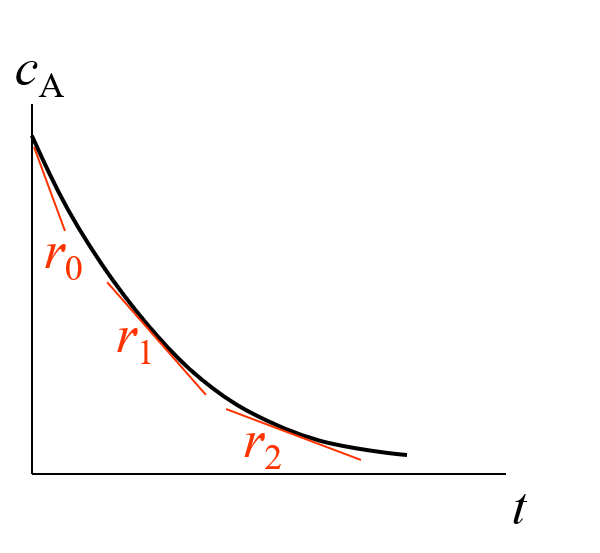
\includegraphics[width=.6\linewidth]{figures/7.1a.png}
                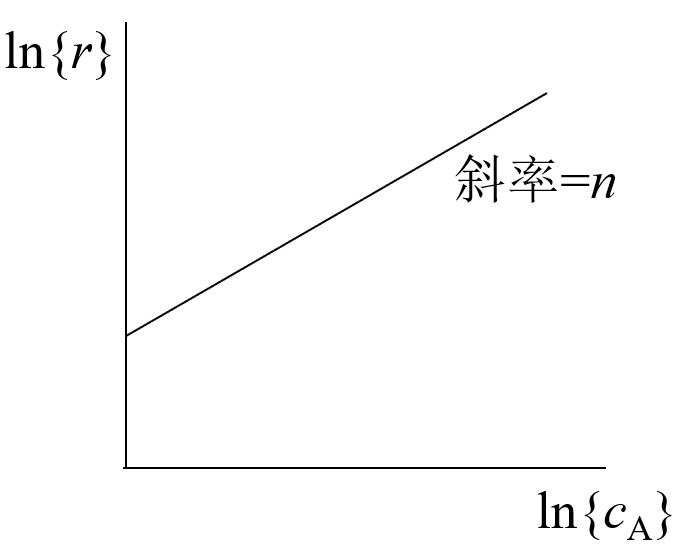
\includegraphics[width=.6\linewidth]{figures/7.1b.png}
            \end{figure}
        \end{minipage}
        
    \end{frame}
    
    
    \begin{frame}
        \frametitle{反应级数的确定}
    
        \begin{itemize}
            \item[3.] \cbf{初速率法(微分法)}
        \end{itemize}
        在反应初始阶段，变化比较简单，复杂的因素较少。只要反应速率不是特别快，可以近似处理，利用初速率求得反应级数。
    
        在不同起始浓度下测定初速率，即在不同起始浓度的$c$-$t$图上求各曲线在$t=0$时的切线斜率$r_0$。再以$\ln r_0$对$\ln c_\mathrm{A0}$作图，所得直线的斜率就是反应级数。
        \begin{figure}
            \centering 
            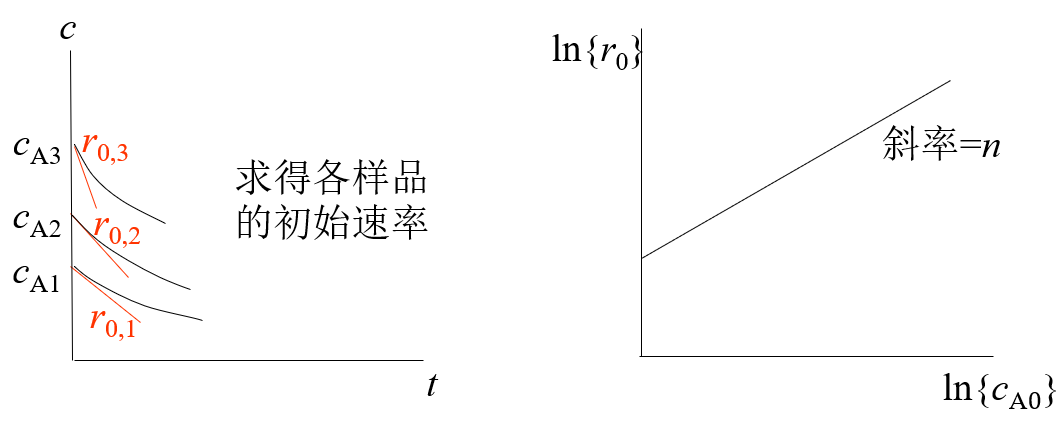
\includegraphics[width=.65\linewidth]{figures/7.2.png}
        \end{figure}
        \vspace{-1pt}
    \end{frame}
    
    
    \begin{frame}
        \frametitle{反应级数的确定}
    
        \begin{itemize}
            \item[4.] \cbf{孤立法}
        \end{itemize}
        \[
            r = k c_\mathrm{A}^\alpha c_\mathrm{B}^\beta
        \]
        当速率方程涉及几种不同物质的浓度时，用上述方法求反应级数就很麻烦。在此情况下，设法将多元函数 $r=f(c_\mathrm{A}, c_\mathrm{B})$在特定条件下变成一元函数，逐个测定$\alpha$、$\beta$。
    
        若反应体系某种物质过量很多，其浓度在反应过程中可以认为没有发生变化，则反应速率只随另一物质的浓度改变。用这种方法可以分别测定该反应对物质A的级数和对B的级数从而测得反应的级数$n = \alpha + \beta$。
    
    \end{frame}


    \section{温度对反应速率的影响}


\begin{frame}
    \frametitle{反应速率与温度的关系}
    \begin{figure}
        \centering 
        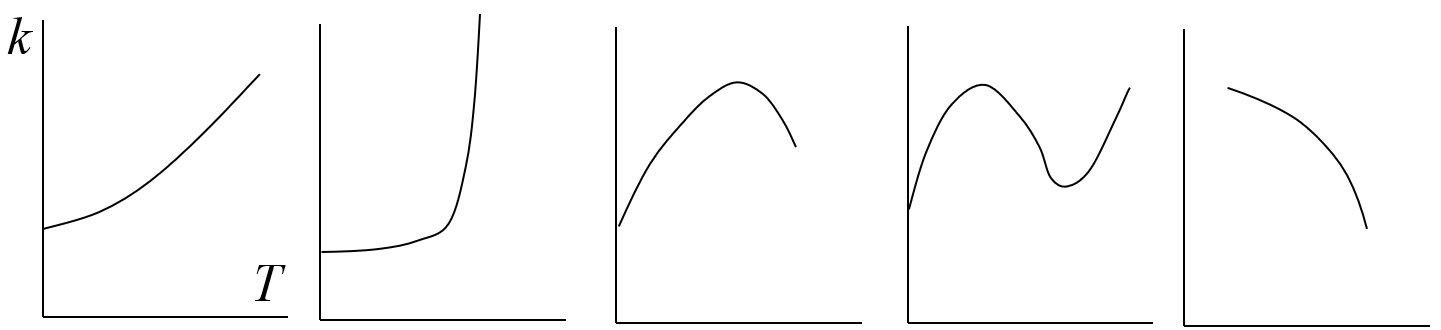
\includegraphics[width=\linewidth]{figures/7.3.png}
    \end{figure}
    \begin{enumerate}
        \item 反应速率随温度升高加快，大多数化学反应的情况
        \item 当温度达到一定极限时，反应高速进行，发生爆炸
        \item 反应速率随温度升高而加快，但超过某一温度后下降
        \item 温度升高时有副反应发生的复杂情况
        \item 反常反应，温度升高，反应速率下降
    \end{enumerate}

\end{frame}


\begin{frame}
    \frametitle{阿伦尼乌斯公式}

    \large 阿伦尼乌斯根据大量的实验事实，提出有关反应速率和温度关系的经验公式
    \[
        k=A \exp \left(\frac{-E_{\mathrm{a}}}{R T} \right)
    \]
    这是阿伦尼乌斯公式的指数式。
    
    \begin{itemize}
        \item $A$是指前因子，又称频率因子，它与碰撞频率有关，是一个重要的动力学参数。单位与$k$相同。$A$是一个经验常数。
        \item $E_a$为活化能 (\si{J.mol^{-1}})        
        \item $R$为摩尔气体常量
    \end{itemize}

\end{frame}


\begin{frame}
    \frametitle{为什么阿伦尼乌斯公式长这样？}
    事实证明，两个粒子相遇并不足以发生反应，它们还必须以足够的能量相互撞击，来跨越一个不稳定的反应障碍（称为过渡态），转化为稳定的反应物状态。这个需要克服的能量被称为活化能$E_a$。根据麦克斯韦-玻尔兹曼能量分布规律，体系中分子总数为$n$时，能量高于$E$值的分子所占的分数为
    \[
        q = \exp (-E/RT)
    \]
    由于我们同时观察这么多的粒子（1摩尔包含\num{6.02e23}个分子），可以使用统计学来考虑，一定比例的粒子将以高于活化能的能量碰撞，而一定比例的能量则以低于活化能的能量碰撞。基于统计热力学和麦克斯韦-玻尔兹曼分布的概念，得出以下关于$k$的温度依赖性的方程：
    \[
        k=A \exp \left(\frac{-E_{\mathrm{a}}}{R T} \right)
    \]
\end{frame}


\begin{frame}
    \frametitle{阿伦尼乌斯公式的其他形式}

    \large 微分式：
    \[
        \frac{\mathrm{d} \ln \{k\}}{\mathrm{d} T}=\frac{E_{\mathrm{a}}}{R T^{2}}
    \]
    定积分式：
    \[
        \ln \frac{k_{2}}{k_{1}}=\frac{-E_{\mathrm{a}}}{R}(\frac{1}{T_{2}}-\frac{1}{T_{1}})
    \]
    不定积分式：
    \[
        \ln {k}=-\frac{E_{\mathrm{a}}}{R} \frac{1}{T}+B
    \]
    上式表明$\ln {k}$与$\frac{1}{T}$之间有线性关系。

\end{frame}


\begin{frame}
    \frametitle{活化能$E_{\mathrm{a}}$}
    \begin{itemize}
        \item 活化能的大小对反应速率影响很大，式中$E_{\mathrm{a}}$出现在指数上就说明了这一点。$E_{\mathrm{a}}$值越小，反应速率越大。
        \item 一般反应活化能约在40～400kJ·mol$^-1$之间, 若$E_{\mathrm{a}}$<40kJ, 反应室温下可瞬时完成; $E_{\mathrm{a}}$>100kJ, 需加热才能完成。
        \item 升高温度对活化能较大的反应影响较大，其反应速率增大的倍数比活化能较小的反应要大得多。
        \item 一般认为$E_{\mathrm{a}}$的大小与温度无关。反应体系温度升高时，活化分子的数量增多，浓度加大，故反应速率增加。
        \item 活化能$E_{\mathrm{a}}$的大小可以通过实验测定。
    \end{itemize}    

\end{frame}


% \begin{frame}[t]
%     \frametitle{}

%     \begin{example}
%         在\SI{0.1}{mol.dm^{-3}}\ch{HCl}水溶液中\ch{(NH2)2CO + H2O -> (NH4)2CO3}，334K时速率常数$k_1=$\SI{0.713e-5}{min^{-1}}，344K时$k_2=$\SI{2.77e-5}{min^{-1}}，求$E_{\mathrm{a}}$和$A$的值。
%     \end{example}

% \end{frame}


\begin{frame}[t]
    \frametitle{}

    \begin{example}
        \ch{CO(CH2COOH)2}在水溶液中的分解反应为一级反应。已知在33K和283K下反应的速率常数分别为\SI{5.48e-2}{s^{-1}}和\SI{1.08e-4}{s^{-1}}，求反应的活化能和在303K下的速率常数。
    \end{example}

\end{frame}


% \begin{frame}[t]
%     \frametitle{}

%     \begin{example}
%         溴乙烷分解反应的活化能$E_{\mathrm{a}}=$\SI{229.3}{kJ.mol^{-1}}，650K时速率常数$k=$\SI{2.14e-4}{s^{-1}}。要使该反应在1 min内完成90\%，反应温度应控制在多少？
%     \end{example}

% \end{frame}

\begin{frame}[t]
    \frametitle{}
    \begin{example}
        某药物溶液若分解30\%即告无效，今测得该药物在323K，333K，343K时的速率常数分别为\SI{7.08e-4}{h^{-1}}，\SI{1.70e-3}{h^{-1}}，\SI{3.55e-3}{h^{-1}}，试计算此反应的活化能以及298K时药物的有效期限。
    \end{example}
\end{frame}


\section{复合反应及近似处理}


\begin{frame}
    \frametitle{复合反应的类型}

    \begin{itemize}
        \item 对峙反应
        \[
            \ch{R <=>[$k+$][$k-$] P}
        \]
        \item 平行反应
        
        \begin{center}
            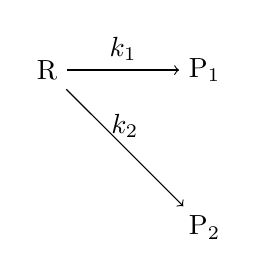
\begin{tikzpicture}
                \node (R) at (0,0) {R};
                \node (P1) at (2,0) {P$_1$};
                \node (P2) at (2,-2) {P$_2$};
                \draw [->] (R) --(P1) node [above,midway] {$k_1$};
                \draw [->] (R) --(P2) node [above,midway] {$k_2$};
            \end{tikzpicture}
        \end{center}

        \item 连串反应
        \[
            \ch{R ->[$k1$] M ->[$k2$] P}
        \]
    \end{itemize}

\end{frame}


\begin{frame}
    \frametitle{对峙反应}

    \[
        \ch{A <=>[$k1$][$k2$] P}
    \]
    \[
        t = 0 \qquad c_\mathrm{A0} \qquad \qquad 0 \qquad \qquad 
    \]
    \[
        t \qquad c_\mathrm{A} \qquad \quad c_\mathrm{A0}-c_\mathrm{A} 
    \]
    \[
        - \frac{\dif c_\mathrm{A} }{\dif t} = k_1 c_\mathrm{A} - k_2 (c_\mathrm{A0} - c_\mathrm{A})
    \]
    \[
        \ln \frac{k_1 c_\mathrm{A0}}{(k_1+k_2)c_\mathrm{A} - k_2c_\mathrm{A0}} = (k_1+k_2)t
    \]
    若$k_1 \gg  k_2$，上式化为$\ln \frac{c_\mathrm{A0}}{c_\mathrm{A}} = k_1t$，为单向一级反应。

    当正逆反应的速率系数相差悬殊时，可以按单向反应处理。

\end{frame}


\begin{frame}
    \frametitle{对峙反应}

    平衡时，
    \[
        k_1 c_\mathrm{A} = k_2 (c_\mathrm{A0} - c_\mathrm{A})
    \]
    可得
    \[
        c_\mathrm{A0} = \frac{k_1 + k_2}{k_2}c_\mathrm{Ae}
    \]
    代入$\ln \frac{k_1 c_\mathrm{A0}}{(k_1+k_2)c_\mathrm{A} - k_2c_\mathrm{A0}} = (k_1+k_2)t$，得
    \[
        \ln \frac{c_\mathrm{A0}-c_\mathrm{Ae}}{c_\mathrm{A}-c_\mathrm{Ae}} = (k_1+k_2)t
    \]
    联立$K = k_1/k_2$，可求得对峙反应的速率常数$k_1$和$k_2$。

    $t$时刻的$c_\mathrm{A}$和平衡时的$c_\mathrm{Ae}$值均可测得，平衡常数$K$可用热力学方法测得。

\end{frame}


\begin{frame}[t]
    \frametitle{}
    \begin{example}
        某1-1级对峙反应\ch{A <=>[$k1$][$k2$] P}，已知$k_1=0.36 \mathrm{min^{-1}}$，$k_2=0.11 \mathrm{min^{-1}}$。若由纯A开始，问经过多长时间后，A与B的浓度相等？
    \end{example}
    \pause
    \[
        \ln \frac{k_1 c_\mathrm{A0}}{(k_1+k_2)c_\mathrm{A} - k_2c_\mathrm{A0}} = (k_1+k_2)t
    \]
    \[
        t = 2.25 \ \mathrm{min}
    \]
\end{frame}


\begin{frame}
    \frametitle{平行反应}

    \[
        \ch{A ->[k1] P} \qquad r_{\mathrm{P}}=k_{1} c_{\mathrm{A}}
    \]
    \[
        \ch{A ->[k2] Q} \qquad r_{\mathrm{Q}}=k_{2} c_{\mathrm{A}}
    \]
    由于各平行反应同时进行，反应的总速率等于各平行反应速率之和。
    \[
        r_\mathrm{A} = r_1 + r_2 = (k_1 + k_2)c_\mathrm{A}
    \]
    \begin{minipage}{0.48\linewidth}
        \[
        \begin{aligned}
            -\frac{\mathrm{d} c_{\mathrm{A}}}{\mathrm{d} t}&=(k_{1}+k_{2}) c_{\mathrm{A}} \\
            \frac{\mathrm{d} c_{\mathrm{P}}}{\mathrm{d} t}&=k_{1} c_{\mathrm{A}}\\
            \frac{\mathrm{d} c_{\mathrm{Q}}}{\mathrm{d} t}&=k_{2} c_{\mathrm{A}}
        \end{aligned}
    \]
    \end{minipage}\hfill
    \begin{minipage}{0.48\linewidth}
        \[
            \begin{aligned}
                c_{\mathrm{A}}&=c_{\mathrm{A} 0} \exp [-(k_{1}+k_{2}) t] \\
                c_{\mathrm{P}}&=\frac{k_{1} c_{\mathrm{A} 0}}{k_{1}+k_{2}}\left\{1-\exp \left[-(k_{1}+k_{2}) t\right]\right\} \\
                c_{\mathrm{Q}}&=\frac{k_{2} c_{\mathrm{A} 0}}{k_{1}+k_{2}}\left\{1-\exp \left[-(k_{1}+k_{2}) t\right]\right\}
            \end{aligned}
        \]
    \end{minipage}

\end{frame}


\begin{frame}
    \frametitle{平行反应}
    \begin{minipage}{0.48\linewidth}
        平行反应中，各反应产物数量之比等于各反应的速率之比。（各反应级数相同，产物起始浓度为零）
    \[
        \frac{c_\mathrm{P}}{c_\mathrm{Q}} = \frac{k_1}{k_2}
    \]
    \end{minipage}\hfill
    \begin{minipage}{0.48\linewidth}
        \begin{figure}[htpb]
            \centering
            
\includegraphics[width=\linewidth]{fig3.2}
        \end{figure}
    \end{minipage}
\end{frame}


\begin{frame}
    \frametitle{连串反应}

    \[
        \ch{R ->[$k1$] M ->[$k2$] P}
    \]
    $$\begin{cases}
        -\frac{\mathrm{d} c_\mathrm{R}}{\mathrm{d} t}   = k_{1} c_\mathrm{R} \\
        \frac{\mathrm{d} c_\mathrm{M}}{\mathrm{d} t} = k_{1} c_\mathrm{R} - k_{2} c_\mathrm{M} \\
        \frac{\mathrm{d} c_\mathrm{P}}{\mathrm{d} t} = k_{2} c_\mathrm{M} 
    \end{cases}$$
    $\begin{aligned}        
        c_\mathrm{R} &=c_\mathrm{R0} \exp (-k_{1} t) \\
        c_\mathrm{M} &=\frac{k_{1} c_\mathrm{R0}}{k_{2}-k_{1}}[\exp (-k_{1} t)-\exp (-k_{2} t)] \\
        c_\mathrm{P} &=c_\mathrm{R0}\left\{1-\frac{k_{2}}{k_{2}-k_{1}}\left[\exp (-k_{1} t)\right]+\frac{k_{1}}{k_{2}-k_{1}}\left[\exp (-k_{2} t)\right]\right\}
    \end{aligned}$

\end{frame}


\begin{frame}
    \frametitle{连串反应}

    \begin{minipage}{0.44\linewidth}
        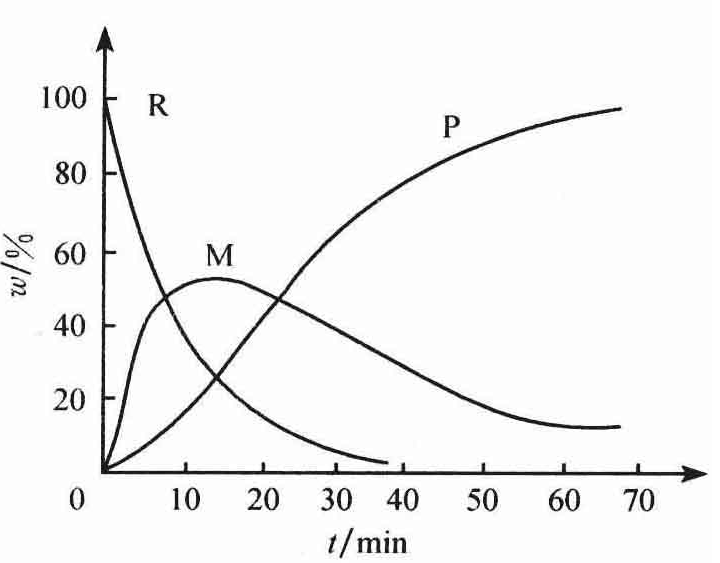
\includegraphics[width=\linewidth]{figures/7.4.png}
    \end{minipage}\hfill
    \begin{minipage}{0.52\linewidth}
        \begin{itemize}
            \item R的浓度逐渐降低
            \item P的浓度逐渐增大
            \item 中间产物M的浓度先增大后降低
        \end{itemize}
    \end{minipage}

    当中间产物M是期望的产品时，必须控制反应时间，在M的浓度达到最大值时终止反应，以期获得最高的产率。
    \[
        t_\mathrm{M_{max}} = \frac{\ln {k_1/k_2}}{k_1 - k_2}
    \]

\end{frame}


\begin{frame}
    \frametitle{复合反应的近似处理}
    化学动力学研究的重要内容之一就是确定反应机理。

    确定复合反应的反应机理是一项艰巨繁杂的任务，但有时可以运用某些近似的处理方法解决复合反应的动力学问题。

    \begin{enumerate}
      \item 速率控制步骤
      \item 平衡假设
      \item 稳态近似
    \end{enumerate}
\end{frame}


\begin{frame}{速率控制步骤}
    \begin{minipage}{0.48\linewidth}
        以反应$\ce{A <=> R}$为例

        各反应步骤均为可逆反应，各反应速率的相对大小如图所示。各反应步骤的正逆反应速率是不相等的，但根据定态近似的假设，其净速率应相等，且等于反应$\ce{A <=> R}$的速率。即
        \[
            r_1=r_2=r
        \]
        第一个反应步骤接近平衡的程度$\frac{\overrightarrow{r}_1-\overleftarrow{r}_1}{\overrightarrow{r}_1}$，远较第二个步骤大，此时第二个步骤便可视为速率控制步骤。
    \end{minipage}\hfill
    \begin{minipage}{0.48\linewidth}
        \begin{figure}[htpb]
            \centering
            
\includegraphics[width=\linewidth]{fig2.5}
        \end{figure}
    \end{minipage}
\end{frame}


\begin{frame}
    \frametitle{平衡假设}
    若在反应过程中包含一个对峙反应，正反应和逆反应的速率都很大，而在该对峙反应之后跟随着一个速率控制的慢反应，就可以近似地认为对峙反应处于平衡状态。

    \medskip
    \begin{minipage}{0.48\linewidth}
        
        第2步为速率控制步骤
        \[
            r_\mathrm{A}=r_\mathrm{A}^*=k_2c_\mathrm{A}^*
        \]
        第1步达到化学平衡
        \[
            c_\mathrm{A}^*c_\mathrm{p}/c_\mathrm{A}=\mathrm{K}_1
        \]
        代入速率方程，得
        \[
            r_\mathrm{A}=k_2\mathrm{K}_1c_\mathrm{A}/c_\mathrm{p}=\mathrm{k}c_\mathrm{A}/c_\mathrm{p}
        \]
        \end{minipage}\hfill
        \begin{minipage}{0.48\linewidth}
            \begin{framed}
            反应\ch{A->P+D}的反应机理如下：
    
            \begin{enumerate}
              \item \ch{A <=> A^* + P}
              \item \ch{A^* -> D}
            \end{enumerate}
            \end{framed}
        \end{minipage}
    
        \smallskip
        $k_2$和$K_1$均为温度的函数，合并为一新的常数$k$，即该反应的反应速率常数。
\end{frame}


\begin{frame}
    \frametitle{稳态近似}
    \begin{minipage}{0.48\linewidth}
        若反应过程达到定态，中间化合物I的浓度就不随时间变化，即
        \[
            \frac{\mathrm{d}c_\mathrm{I}}{\mathrm{d}t}=0
        \]
        也可以说，若达到定态，则串联进行的各反应步骤速率相等。这两种说法是一样的。
    \end{minipage}\hfill
    \begin{minipage}{0.48\linewidth}
        设化学反应$\ce{A <=> R}$由下列两个步骤构成
        \[
            \mathrm{A} \rightleftharpoons \mathrm{A∗} \qquad r_1=\overrightarrow{k}_1c_\mathrm{A}-\overleftarrow{k}_1c_\mathrm{A}
        \]
        \[
            \mathrm{A∗} \rightleftharpoons \mathrm{R} \qquad r_2=\overrightarrow{k}_2c_\mathrm{A}-\overleftarrow{k}_2c_\mathrm{A}
        \]
        中间化合物$\mathrm{A∗}$的浓度变化速率为
        \[
            \begin{aligned}
                \frac{\mathrm{d}c_\mathrm{A∗}}{\mathrm{d}t}&=r_1-r_2 \\
                &=(\overrightarrow{k}_1c_\mathrm{A}-\overleftarrow{k}_1c_\mathrm{A})-(\overrightarrow{k}_2c_\mathrm{A}-\overleftarrow{k}_2c_\mathrm{A})
            \end{aligned}
        \] 
    \end{minipage}
\end{frame}


\begin{frame}
    \frametitle{稳态近似}
    若反应过程达到定态，中间化合物I的浓度就不随时间变化，即$\frac{\mathrm{d}c_\mathrm{I}}{\mathrm{d}t}=0$。
    
    也可以说，若达到定态，则串联进行的各反应步骤速率相等。这两种说法是一样的。

    设化学反应$\ce{A <=> R}$由下列两个步骤构成
        \[
            \mathrm{A} \rightleftharpoons \mathrm{A∗} \qquad r_1=\overrightarrow{k}_1c_\mathrm{A}-\overleftarrow{k}_1c_\mathrm{A}
        \]
        \[
            \mathrm{A∗} \rightleftharpoons \mathrm{R} \qquad r_2=\overrightarrow{k}_2c_\mathrm{A}-\overleftarrow{k}_2c_\mathrm{A}
        \]
        中间化合物$\mathrm{A∗}$的浓度变化速率为
        \[
            \begin{aligned}
                \frac{\mathrm{d}c_\mathrm{A∗}}{\mathrm{d}t}&=r_1-r_2 \\
                &=(\overrightarrow{k}_1c_\mathrm{A}-\overleftarrow{k}_1c_\mathrm{A})-(\overrightarrow{k}_2c_\mathrm{A}-\overleftarrow{k}_2c_\mathrm{A})
            \end{aligned}
        \] 
\end{frame}


\section{催化剂}


\begin{frame}
    \frametitle{催化剂和催化作用}
    大多数工业反应都要通过催化作用。催化反应的基本特征有：
    \begin{itemize}
        \item[1] 催化剂的存在改变了反应途径。在催化反应中，催化剂与反应物形成活性配合物，然后活性配合物再生产反应产物，同时释放出催化剂，使催化剂能继续使用。
        \item[2] 催化剂只能改变达到平衡的时间，不能改变反应物系最终能达到的平衡状态。
        \item[3] 催化剂具有选择性。
    \end{itemize}
    \begin{blankblock}{}
        乙醇分解反应，采用酸催化剂如$\gamma$-\ch{Al2O3}时，进行的是脱水反应
        \[
            \ch{C2H5OH -> C2H4 + H2O}
        \]
        采用金属催化剂，如铜催化剂，得到的产物不再是乙烯，而是脱氢生成乙醛：
        \[
            \ch{C2H5OH -> CH3CHO + H2}
        \]
    \end{blankblock}
\end{frame}


\begin{frame}
    \frametitle{催化剂和催化作用}
    \begin{itemize}
        \item[4] 催化剂不改变化学反应的可能性。
        
        对于热力学上不可能的反应，任何催化剂都不能使之发生。
        \item[5] 催化剂对某些杂质很敏感。
            \begin{itemize}
              \item 增强催化作用的杂质可称为助催化剂
              \item 减弱催化作用的杂质称为抑制剂
              \item 使催化剂完全失去催化功能的杂质称为毒物。
            \end{itemize}
        \item[6] 反应过程中催化剂的变化
            \begin{itemize}
              \item 反应前后催化剂本身的数量不变
              \item 但有些形状，特别是固体催化剂表面性状会发生变化。
            \end{itemize}
    \end{itemize}
\end{frame}


\begin{frame}{固体催化剂}
    固体催化剂绝大多数为颗粒状，一般情况下，固体催化剂由三部分组成：
    \begin{itemize}
      \item 主催化剂：起催化作用
      \item 助催化剂：含量一般很少，其作用主要是提高催化剂的催化活性、选择性和稳定性。
      \item 载体：多孔结构，增大表面积
    \end{itemize}
    
    \begin{blankblock}{}
        不同的反应对比表面有不同的要求。比表面大就意味着载体的孔半径小，从而增大了扩散阻力。
        \begin{itemize}
          \item $\alpha$-\ch{Al2O3} \quad $1\sim 10$ \si{m^2/g}。
          \item $\gamma$-\ch{Al2O3}  \quad  $100\sim 300$ \si{m^2/g}。
          \item 活性炭 \quad \ $500\sim 1500$ \si{m^2/g}。
        \end{itemize}
    \end{blankblock}
\end{frame}


\begin{frame}{多相催化反应步骤}
    \begin{minipage}{0.48\linewidth}
        气态或液态反应物在固态催化剂表面发生的催化反应为多相催化反应。

        多相催化反应由下列步骤所构成：
        \begin{enumerate}
          \item 外扩散
          \item 内扩散
          \item 吸附
          \item 表面反应
          \item 脱附
          \item 内扩散
          \item 外扩散
        \end{enumerate}
    \end{minipage}\hfill
    \begin{minipage}{0.48\linewidth}
        \begin{figure}[htpb]
            \centering
            
\includegraphics[width=\linewidth]{fig6.1}
        \end{figure}
    \end{minipage}
\end{frame}















\end{document}